\documentclass{article}

% if you need to pass options to natbib, use, e.g.:
%     \PassOptionsToPackage{numbers, compress}{natbib}
% before loading neurips_2018

% ready for submission
% \usepackage{neurips_2018}

% to compile a preprint version, e.g., for submission to arXiv, add add the
% [preprint] option:
    \usepackage[preprint]{neurips_2018}

% to compile a camera-ready version, add the [final] option, e.g.:
    %  \usepackage[final]{neurips_2018}

% to avoid loading the natbib package, add option nonatbib:
    % \usepackage[nonatbib]{neurips_2018}

\usepackage[utf8]{inputenc} % allow utf-8 input
\usepackage[T1]{fontenc}    % use 8-bit T1 fonts
\usepackage{hyperref}       % hyperlinks
\usepackage{url}            % simple URL typesetting
\usepackage{booktabs}       % professional-quality tables
\usepackage{amsfonts}       % blackboard math symbols
\usepackage{nicefrac}       % compact symbols for 1/2, etc.
\usepackage{microtype}      % microtypography
\usepackage{ctex}
\usepackage{graphicx}
\usepackage{amsmath}

\title{对抗样本不是缺陷,而是特征}

% The \author macro works with any number of authors. There are two commands
% used to separate the names and addresses of multiple authors: \And and \AND.
%
% Using \And between authors leaves it to LaTeX to determine where to break the
% lines. Using \AND forces a line break at that point. So, if LaTeX puts 3 of 4
% authors names on the first line, and the last on the second line, try using
% \AND instead of \And before the third author name.

\author{%
  Andrew Ilyas \\
  MIT\\
  \texttt{ailyas@mit.edu} \\
  \And
  Shibani Santurkar \\
  MIT \\
  \texttt{shibani@mit.edu} \\
  \And
  Dimitris Tsipras \\
  Affiliation \\
  \texttt{tsipras@mit.edu} \\
  \AND
  Logan Engstrom \\
  MIT \\
  \texttt{engstrom@mit.edu} \\
  \And
  Brandon Tran \\
  MIT \\
  \texttt{btran115@mit.edu} \\
  \And
  Aleksander Mądry \\
  MIT \\
  \texttt{madry@mit.edu} \\
}

\begin{document}
% \nipsfinalcopy is no longer used

\maketitle
\begin{abstract}
  对抗样本在机器学习中引起了广泛关注,但其存在性和普遍性的原因尚不清楚。我们证明,对抗样本可以直接归因于非鲁棒特征的存在:来自数据分布模式的特征具有很强的预测性,但对人类来说是脆弱和不可理解的。在理论框架内捕获这些特征之后,我们在标准数据集中证明了它们的广泛存在。最后,我们提出了一个简单的设置,在这个设置中,我们可以严格地将我们在实践中观察到的现象与(人类指定的)鲁棒性概念和数据的固有几何结构之间的偏差联系起来。
\end{abstract}

\section{引言}

深部神经网络的普遍脆弱性近年来引起了人们的极大关注。尤其令人担忧的是对抗样本的现象[Big+13;Sze+14],被不可察觉的噪声扰动后自然输入,在最先进的分类器中引起错误的预测。以前的工作已经对这种现象提出了各种解释,从理论模型[sch+18;bpr18]到基于高维测度的观点[gil+18;mdm18;sha+19a]。然而,这些理论往往无法完全捕捉我们在实践中观察到的行为(我们将在第5节中进一步讨论这一点)。

\ \ \ \ 更广泛地说,以前在该领域的工作往往将对抗样本视为输入空间的高维性质或训练数据的统计波动引起的畸变[sze+14;gss15;gil+18]。从这个角度来看,很自然地将对抗性稳健性视为一个可以被解纠缠的目标,通过改进的标准正则化方法[TG16]或对网络输入/输出的前/后处理[UES+18;CW17A;HE+17],可以独立地追求精度最大化[MAD+18;SHS19;SUG+19]。

\ \ \ \ 在这项工作中,我们基于对抗样本的现象提出了一个新的观点。与之前的模型相比,我们将对抗脆弱性视为主流监督学习范式的基本结果。具体来说,我们认为:
\begin{center}
  \textit{对抗脆弱性是我们的模型对数据中能够很好泛化的特征的敏感性的直接结果。}
\end{center}
回想一下,我们通常训练分类器来单独最大化(分布)精度。因此,分类器倾向于使用任何可用的信号来实现这一点,即使是那些看起来人类无法理解的信号。毕竟,“尾巴”或“耳朵”的出现对于分类器来说并不比任何其他同等的预测模式更自然。事实上,我们发现标准的机器学习数据集确实包含高度预测但不可察觉的模式。我们假设我们的模型学习依赖于这种模式产生的“非鲁棒”特征,从而导致利用这种依赖性的对抗扰动。

\ \ \ \ 我们的假设也为对抗迁移性提供了一种解释:从一个模型计算出的对抗性扰动通常可以迁移到另一个独立训练的模型上。由于任何两个模型都可能学习类似的非鲁棒特征,因此操纵这些特征的扰动将同时适用于这两个模型。最后,这种观点将对抗性脆弱性确立为一种纯粹的以人为中心的现象,因为从标准监督学习的角度来看,非鲁棒性特征与鲁棒性特征一样重要。它还表明,旨在通过对给定模型的解释实施“先验”[erh+09;mv15;oms17]来增强该模型的可解释性的方法实际上隐藏了“有意义”和对标准模型具有预测性的特征。因此,不能独立于模型本身的训练来寻求对模型忠诚而又对人类有意义的解释。

为了证实我们的理论,我们证明了在标准图像分类数据集中区分鲁棒性和非鲁棒性是可能的。具体来说,对于任何训练数据集,我们都能够构建:
\begin{enumerate}
  \item \textbf{用于鲁棒分类的鲁棒化版本(图\ref{fig:1}a)。}我们证明了从数据集中有效地删除非鲁棒特征是可能的。具体来说,我们创建了一个训练集(语义上类似于原始的),在这个训练集上,标准训练在原始的、未修改的测试集上产生良好的鲁棒精度。这一发现表明,对抗性脆弱性不一定与标准培训框架挂钩,而是数据集的一个属性。
  \item \textbf{用于标准分类的非鲁棒版本(图\ref{fig:1}b)。}我们还可以构建一个训练数据集,其输入几乎与原始数据集相同,但所有数据集的标签都不正确。事实上,新训练集中的输入的标签与其被添加对抗性扰动对应(因此仅使用非鲁棒特征)。尽管缺乏任何可预测的人类可见信息,但在这个数据集上的训练在原始的、未修改的测试集上产生了良好的准确性。
\end{enumerate}

\ \ \ \ 最后,我们提出了一个具体的分类任务,在这个任务中,可以严格研究对抗样本与非鲁棒性特征之间的关系。这项任务包括分离高斯分布,并松散地基于Tsipras等人提出的模型。[TSI+19],同时以一些方式扩展它。首先,我们设置中的对抗脆弱性可以精确地量化为内在数据几何结构与对手扰动集之间的差异。第二,鲁棒训练产生一个分类器,该分类器充分利用这两者组合对应的几何体。最后,标准模型的梯度可以明显地与类间方向更不一致,以捕捉在更复杂的场景中实际观察到的现象[TSI+19]。

\begin{figure}[h]
  \centering
  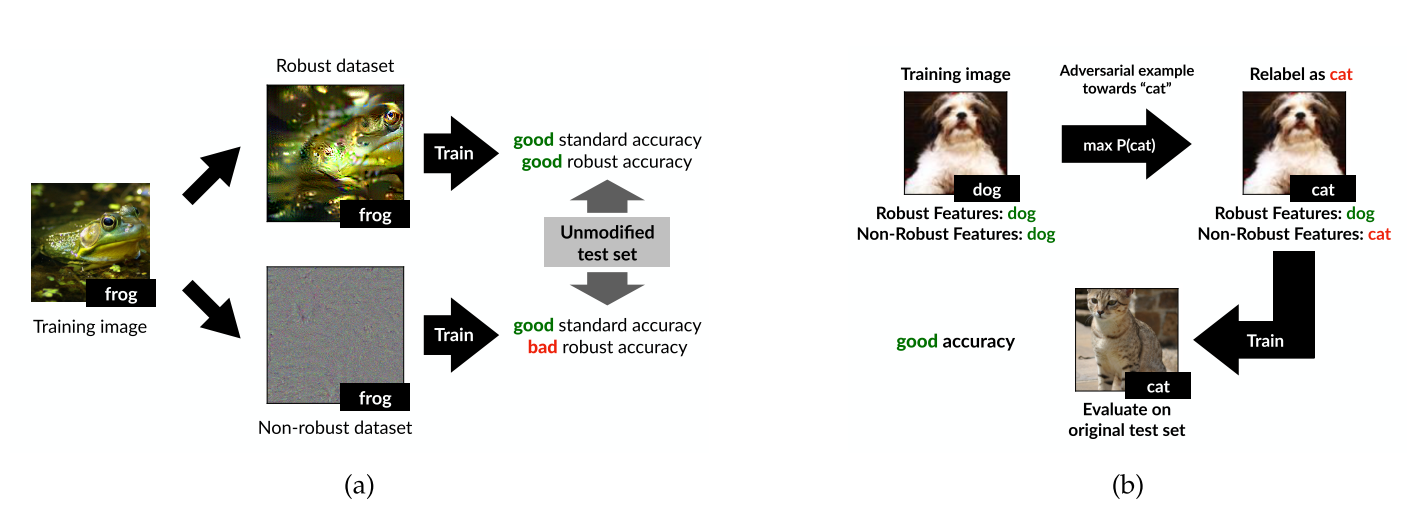
\includegraphics[width=13cm]{fig/figure1.png}
  \caption{第3节实验的概念图。在(a)中,我们将特征分为鲁棒/非鲁棒特征的组合。在(b)中,我们构建了一个数据集,该数据集在人类看来是错误的(通过对抗样本),但在最初的测试集上具有良好的准确性。}
  \label{fig:1}
\end{figure}

\section{鲁棒特征模型}  \label{section:2}

我们首先开发了一个框架,大致基于Tsipras等人提出的设置[TSI+19],使我们能够严格地操纵“鲁棒”和“非鲁棒”特征。特别地,我们提出了一套定义,允许我们正式描述我们的设置、理论结果和经验证据。

\textbf{设置。}我们考虑二分类问题,它的输入和标签 $(x, y) \in \mathcal{X} \times\{ \pm 1\}$ 是从(数据)分布 $\mathcal{D}$ 中采样的。目标是学习一个分类器 $C : \mathcal{X} \rightarrow\{ \pm 1\}$ ,它可以为给定输入 $x$ 预测一个标签 $y$ 。

\ \ \ \ 我们定义特征为一个从输入空间 $\mathcal{X}$ 到实数的一个函数映射,所有的特征集合为 $\mathcal{F}=\{f : \mathcal{X} \rightarrow \mathbb{R}\}$ 。方便起见,为了使的后面的定义具有尺度不变性,我们假设在$\mathcal{F}$中的特征被放缩至均值为零且方差为一(比如 $\mathbb{E}_{(x, y) \sim \mathcal{D}}[f(x)]=0$ 且 $\mathbb{E}_{(x, y) \sim \mathcal{D}}\left[f(x)^{2}\right]=1$)。注意,这个形式化的定义也捕获了我们抽象地认为的特征(例如,我们可以构造一个$f$来捕获一个图像是如何“毛茸茸的”)。

\textbf{有用的、鲁棒的和非鲁棒的特征。}现在,我们定义了制定框架所需的关键概念。为此,我们按以下方式对特征进行分类:
\begin{itemize}
  \item \textbf{$\rho$-有用特征:}对于给定的分布$D$,我们称一个特征$f$是$\rho$-有用的($\rho 》 0$),如果它在期望上与真实的标签相关,即
  \begin{equation}
    \mathbb{E}_{(x, y) \sim \mathcal{D}}[y \cdot f(x)] \geq \rho.
  \end{equation}
  我们定义$\rho_{\mathcal{D}}(f)$为分布$D$下最大的$\rho$,这里特征$f$是$\rho$-有用的。(注意,如果一个特征$f$是与标签负相关的,则$-f$将被使用。)关键地,一个在$\rho$-有用特征上训练过的线性分类器可以获得非平凡的泛化性能。
  \item \textbf{$\gamma$-鲁棒有用特征:}假设我们有一个$\rho$-有用特征$f\left(\rho_{\mathcal{D}}(f)>0\right)$。我们称$f$为鲁棒特征(正式地说,一个$\gamma$-鲁棒有用特征,当$\gamma > 0$),如果在对抗扰动(对某些特定的有效的扰动$\Delta$)下$f$依然是$\gamma$-有用的。正式地,如果我们有
  \begin{equation}
    \mathbb{E}_{(x, y) \sim \mathcal{D}}\left[\inf _{\delta \in \Delta(x)} y \cdot f(x+\delta)\right] \geq \gamma.
  \end{equation}
  \item \textbf{有用不鲁棒特征:}一个有用但不鲁棒的特征是指,该特征对于某些有界且大于零的$\rho$是$\rho$-有用的,但对任何$\gamma \geq 0$却不是一个$\gamma$-鲁棒有用特征。这些特征在标准设置中对分类有益,但是可能会阻碍对抗设置中的精度,因为标签的相关性可能会被翻转。
\end{itemize}

\textbf{分类。}在我们的框架中,一个分类器 $C=(F, w, b)$ 由一个特征集合 $F \subseteq \mathcal{F}$ 、一个权重向量 $w$ 和一个偏置标量 $b$ 组成。对于一个给定的输入$x$,分类器预测的标签$y$表示为
\begin{equation*}
  C(x)=\textnormal{sgn}\left(b+\sum_{f \in F} w_{f} \cdot f(x)\right). 
\end{equation*}
方便起见,我们将一个分类器$C$学习到的特征集合记为$F_{C}$。

\textbf{标准训练。}训练分类器是通过最小化损失函数(通过经验风险最小化(ERM))来完成的,损失函数随特征的加权组合和标签之间的相关性增加而减小。这种损失最简单的一个例子是
\begin{equation}
  \mathbb{E}_{(x, y) \sim \mathcal{D}}\left[\mathcal{L}_{\theta}(x, y)\right]=-\mathbb{E}_{(x, y) \sim \mathcal{D}}\left[y \cdot\left(b+\sum_{f \in F} w_{f} \cdot f(x)\right)\right]
\end{equation}
当分类损失最小化时,鲁棒特征和非鲁棒特征之间不存在区别:特征的唯一区别因素是其$\rho$-有用性。此外,分类器将利用$F$中的任何$\rho$-有用特征来减少分类器的损失。

\textbf{鲁棒训练。}在存在敌人的情况下,任何有用但不鲁棒的特征都可以与真正的标签反相关,从而导致对抗脆弱性。因此,ERM不再足以训练鲁棒的分类器,我们需要明确考虑对手对分类器的影响。为了做到这一点,我们使用了一种对抗性的损失函数,它可以区分稳健和非稳健特征[MAD+18]:
\begin{equation}
  \mathbb{E}_{(x, y) \sim \mathcal{D}}\left[\max _{\delta \in \Delta(x)} \mathcal{L}_{\theta}(x+\delta, y)\right],
\end{equation}
对于一个适当定义的扰动$\Delta$。由于对手可以利用非鲁棒特征来降低分类精度,因此可以将这种对抗性损失(如在对抗性训练中[GSS15;MAD+18])视为明确地阻止分类器学习有用但非鲁棒的特征组合。

\section{寻找鲁棒(非鲁棒)特征}

我们提出的框架的中心前提是既存在鲁棒性特征又存在非鲁棒性特征,这些特征构成了标准分类的有用信号。我们现在通过分离这两组特征来提供支持这一假设的证据。

\ \ \ \ 一方面,我们将构建一个“鲁棒化”的数据集,由主要包含鲁棒特征的样本组成。使用这样一个数据集,我们能够使用标准(即非鲁棒)训练来训练鲁棒的分类器(对于标准测试集)。这表明,通过从数据集中删除某些特征(总的来说,新数据集包含的信息相对于原始训练集较少),可以产生鲁棒性。此外,它还提供了证据,证明对抗脆弱性是由非鲁棒特征造成的,并且与标准训练框架没有内在联系。

\ \ \ \ 另一方面,我们将构建一个数据集,其中输入和标签的关联纯粹基于非健壮特征(因此,相应的数据集对于人类来说似乎完全错误地被标记)。我们证明这个数据集足以训练一个在标准测试集上具有良好性能的分类器。这表明自然模型使用非鲁棒特征来进行预测,即使存在鲁棒特征。这些特征本身就足以满足自然图像的非平凡的泛化性能,这表明它们确实是有价值的特征,而不是有限样本过拟合的产物。

\ \ \ \ 这些实验的概念性的描述请参见图\ref{fig:1}。

\subsection{区分鲁棒和非鲁棒的特征}

回想一下,分类器学习去依靠的特征仅仅是基于这些特征对泛化性是否有用。
因此,在我们的概念框架下,如果我们能够确保只有鲁棒的特征是有用的,那么标准训练应该会产生一个鲁棒的分类器。不幸的是,我们不能直接操纵非常复杂的高维数据集的特征。相反,我们将利用一个鲁棒的模型来修改我们的数据集,使其只包含与该模型相关的特征。

\ \ \ \ 根据我们的正式框架(第\ref{section:2}节),给定一个鲁棒(比如,对抗训练)的模型$C$,我们可以构建一个分布$\widehat{\mathcal{D}}_{R}$,使其满足:
\begin{equation}
\label{equation:5}
\mathbb{E}_{(x, y) \sim \widehat{\mathcal{D}}_{R}}[f(x) \cdot y]=\left\{
  \begin{array}{ll}
    {\mathbb{E}_{(x, y) \sim \mathcal{D}}[f(x) \cdot y]} & {\text { if } f \in F_{C}} \\ {0} & {\text { otherwise, }}
  \end{array}\right.
\end{equation}
其中$F_C$表示$C$使用的特征集合。概念上,我们希望$C$使用的特征像原始分布$\mathcal{D}$上的特征一样有用,同时确保在$\widehat{\mathcal{D}}_{N R}$中其余的特征无用。

我们将为$\widehat{\mathcal{D}}_{R}$构建一个训练集,通过从原始训练集$\mathcal{D}$中 $x \mapsto x_{r}$ 的一对一的映射。在深度神经网络的情况下,$F_C$恰好对应于网络倒数第二层(因为接下来将被输入至一个线性分类器)的激活特征集合。为了确保模型使用的特征在两个数据集下同样有用,我们(近似地)使$F_C$中所有特征对$x$和$x_r$具有相近的值,通过优化下式:
\begin{equation}
\label{equation:6}
  \min _{x_{r}}\left\|g\left(x_{r}\right)-g(x)\right\|_{2}
\end{equation}
其中$x$是原始的输入,$g$是从$x$到表示层的映射。我们使用梯度下降在输入空间优化该目标。

\ \ \ \ 因为我们并不能直接访问除$F_C$之外的特征,所以没有办法使得式\eqref{equation:5}中对于所有 $f \notin F_{C}$ 的期望为零。为了达到这个目的,我们选择从$\mathcal{D}$中独立于$x$的标签抽取一个输入$x_0$,作为式\eqref{equation:6}中优化问题的初始点。这个选择确保了该输入的任何特征都没有用因为它们的期望与标签不相关。这里一个潜在的假设是,在式\eqref{equation:6}中执行优化时,未直接优化的特征(即$F_C$之外的特征)不会受到影响。

\ \ \ \ 给定$\widehat{\mathcal{D}}_{R}$的一个新的训练集(一些随机样本在图\ref{fig:2}a中展示),我们使用标准(非鲁棒)训练来训练一个分类器。我们在原始的测试集(即$\mathcal{D}$)上特使这个分类器。结果(图\ref{fig:2}b)显示,使用新数据集学习到的分类器在在标准设置和对抗设置下都有不错的精度。

\begin{figure}[h]
  \centering
  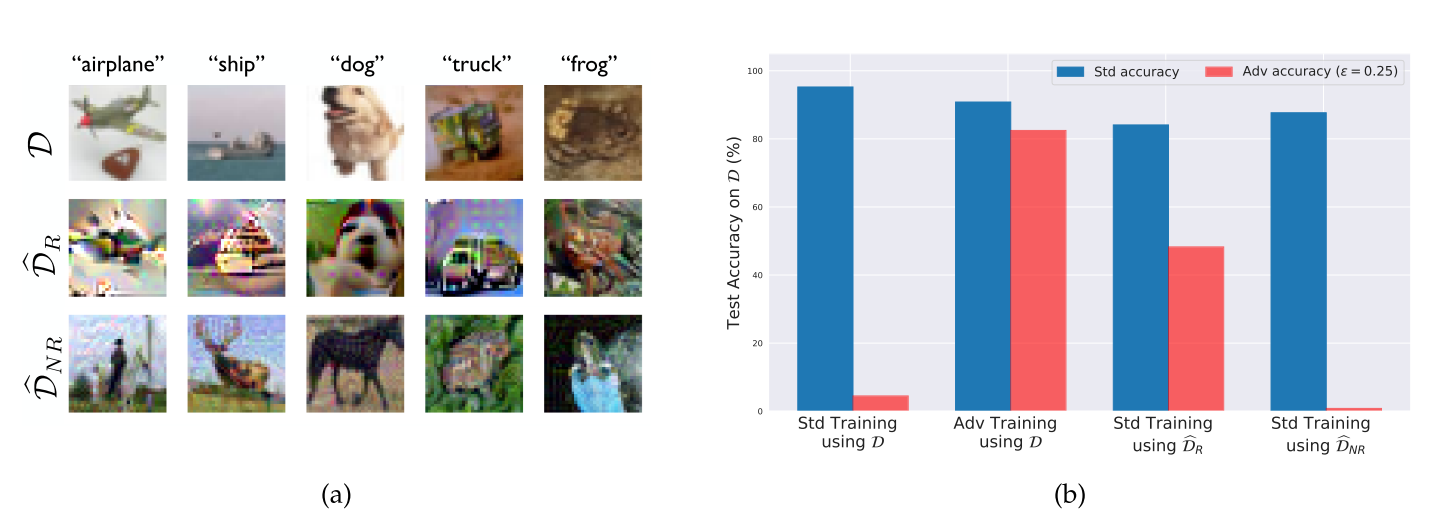
\includegraphics[width=13cm]{fig/figure2.png}
  \caption{\textbf{左图:}我们CIFAR-10[Kri09]训练集的变种中的随机样本:原始训练集$\mathcal{D}$;鲁棒训练集$\widehat{\mathcal{D}}_{R}$,仅仅包含鲁棒模型使用的特征;非鲁棒训练集$\widehat{\mathcal{D}}_{N R}$,仅仅使用与标准 模型相关的特征(标记对人类来说是不正确的)。\textbf{右图:}模型在CIFAR-10测试集($\mathcal{D}$)上的标准和鲁棒精度:(i)在$\mathcal{D}$上标准训练;(ii)在$\widehat{\mathcal{D}}_{N R}$上标准训练;(iii)在$\mathcal{D}$上对抗训练;(iv)在$\widehat{\mathcal{D}}_{R}$上标准训练。在 $\widehat{\mathcal{D}}_{R}$ 和 $\widehat{\mathcal{D}}_{NR}$ 上训练的模型表明用于创建它们的原始模型:值得注意的是,在 $\widehat{\mathcal{D}}_{R}$ 上的标准训练带来了不平凡的鲁棒精度。}
  \label{fig:2}
\end{figure}

\ \ \ \ 作为对照,我们在构建数据集时使用一个标准(非鲁棒)模型重复此方法。图\ref{fig:2}a展示了所得到的“非鲁棒数据集” $\widehat{\mathcal{D}}_{NR}$ 的一些样本——它们更像优化中的源图$x_0$而不是目标图$x$。我们发现在这个数据集上训练可以得到较好的标准精度,却几乎没有鲁棒性(\ref{fig:2}b)。我们还验证了这个过程不仅仅是在对原始模型的权重进行重新编码——如果我们使用与原始模型不同的架构进行训练,在 $\widehat{\mathcal{D}}_{R}$ 和  $\widehat{\mathcal{D}}_{NR}$上都会得到相同的结果。

\subsection{非鲁棒特征足以进行标准分类}

上一节的结果表明,通过将数据集限制为仅包含鲁棒模型所使用的特征,标准训练将导致分类器具有鲁棒性。这表明,在对标准数据集进行训练时,非鲁棒特征在所得到的学习分类器中起着很大的作用。
在这里,我们开始证明这个现象不仅仅是偶然的,也不是由于有限样本的过拟合。特别地,我们证明了仅非鲁棒特征就足以实现标准泛化——即,仅对非鲁棒特征进行训练的模型可以在标准测试集上表现良好。

\ \ \ \ 为了证明这一点,我们构建了一个数据集,其中对分类有用的唯一特征是非鲁棒特征(或根据第二节中的正式模型,所有的$\rho$-有用的特征$f$都是不鲁棒的)。为此,我们修改每个输入标签对$(x, y)$,如下所示。我们选择一个目标类别$t$,要么(a)在类之间均匀随机选择,要么(b)根据源类确定(例如,对标签进行固定的置换)。然后,我们在x上加上一个小的对抗扰动,以确保它被标准模型分类为$t$。正式地:
\begin{equation}
  x_{a d v}=\underset{\left\|x^{\prime}-x\right\| \leq \varepsilon}{\arg \min } \ L_{C}\left(x^{\prime}, t\right)
\end{equation}
其中$L_C$是标准(非鲁棒)分类器$C$的损失函数,$\epsilon$是一个较小的常数。对于一个人类观察者来说,得到的输入几乎与原始没有区别,因此被赋予到修改后的输入的标签$t$似乎是不正确的。得到的输入标签对$(x_{adv}, t)$组成了新的数据集。

\ \ \ \ 现在,因为$\left\|x_{a d v}-x\right\|$很小,根据定义$x_{adv}$的鲁棒特征仍然与类标签$y$(而不是$t$)相关,在整个数据集的期望上。毕竟,人类仍然识别出原始类别。另一方面,由于每个$x_{adv}$都被标准分类器强烈地判别为$t$,因此一定有一些非鲁棒的特征现在与类别$t$非常相关(在期望上)。因此,对于任何一个$t$(不论是随机的还是确定式的),仅仅新数据集的非鲁棒特征与新标记协同。

\ \ \ \ 当$t$是随机选择的时,鲁棒特征(期望上)与标记$t$不相关,因此对分类无用。正式地,我们旨在构建一个数据集$\widehat{\mathcal{D}}_{\text {rand}}$使得:
\begin{equation}
\mathbb{E}_{(x, y) \sim \widehat{D}_{\text {rand}}}[y \cdot f(x)] \left\{\begin{array}{ll}{>0} & {\text { if } f \text { non-robustly useful under } \mathcal{D},} \\ {=0} & {\text { otherwise. }}\end{array}\right.
\end{equation}
当$t$是决定式地基于$y$选择的,鲁棒特征实际上背离指定的标签$t$。实际上,所有的被标记为$t$的输入表现出非鲁棒与$t$相关,而鲁棒特征与原始类别$y$相关。因此,原始训练集上的鲁棒特征提供了意义非凡的预测能力,但实际上伤害了在标准测试集上的泛化能力。使用正式模型的角度看待这个情况,我们的目标是构建一个数据集$\widehat{\mathcal{D}}_{d e t}$使得:
\begin{equation}
\mathbb{E}_{(x, y) \sim \widehat{D}_{d e t}}[y \cdot f(x)] \left\{\begin{array}{ll}{>0} & {\text { if } f \text { non-robustly useful under } \mathcal{D}} \\ {<0} & {\text { if } f \text { robustly useful under } \mathcal{D}} \\ {\in \mathbb{R}} & {\text { otherwise }(f \text { not useful under } \mathcal{D})}\end{array}\right.
\end{equation}

\ \ \ \ 我们发现在这些数据集上的标准训练实际上在原始的测试集上泛化得很好,如表\ref{table:1}所示。
\begin{table}
  \centering
  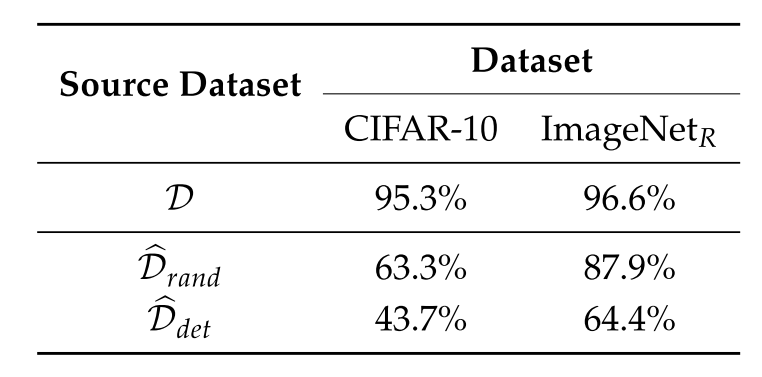
\includegraphics[width=8cm]{fig/table1.png}
  \caption{在使用标准模型创造的训练集$\mathcal{D}$、$ \widehat{\mathcal{D}}_{\text {rand}}$ 和 $\widehat{\mathcal{D}}_{\text {det}}$上训练的分类器的测试精度(在$\mathcal{D}$上)。对于$ \widehat{\mathcal{D}}_{\text {rand}}$ 和 $\widehat{\mathcal{D}}_{\text {det}}$,只有非鲁棒的特征是有用的特征。这些数据集是使用从$x$到类别$t$的对抗扰动构造的;得到的图片被重新标记为$t$。}
  \label{table:1}
\end{table}

\subsection{迁移性可能来自非鲁棒特征}

对抗样本最有趣的特性之一是,它们可以在具有不同架构和独立采样的训练集的模型之间迁移[Sze+14;PMG16;CRP19]。在这里,我们表明,这一现象实际上可以被视为非鲁棒特征存在的自然结果。回想一下,根据我们的主要理论,对抗样本是对可泛化却脆弱的特征进行扰动的结果。鉴于这些特征是数据分布的固有特征,对来自该分布的独立样本进行训练的不同分类器可能会使用相似的非鲁棒特征。因此,通过利用一个分类器学习到的非鲁棒特征构建的一个对抗样本将以类似的方式迁移到其它的任何一个使用这些特征的分类器上。

\begin{figure}
  \centering
  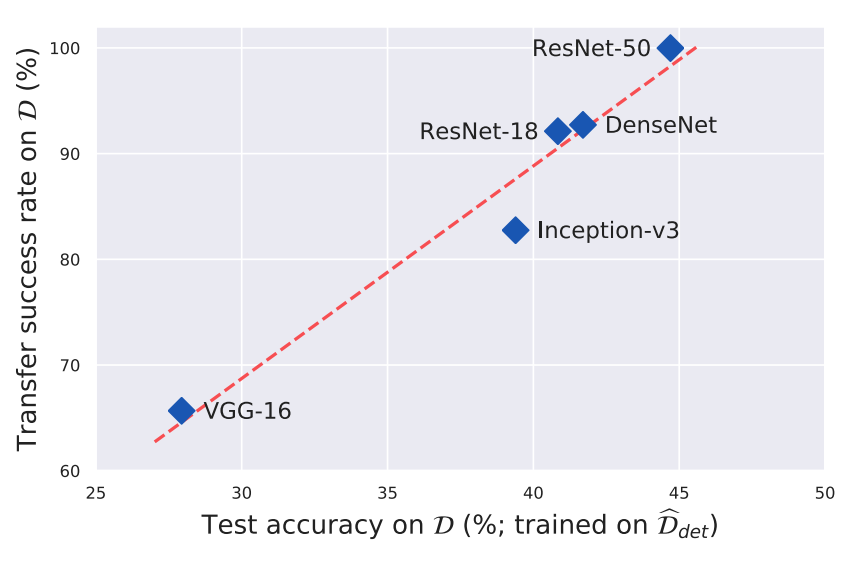
\includegraphics[width=11cm]{fig/figure3.png}
  \caption{从ResNet-50到不同架构网络的迁移成功率与这些架构的测试精度,它们都是在第3.2节生成的数据集上训练的。对迁移攻击更脆弱的架构同时在标准测试集上表现得更好,这一现象支撑了我们的假设:对抗迁移性是由利用了相似的非鲁棒特征引起的。}
  \label{figure:3}
\end{figure}

\ \ \ \ 为了说明和证实这一假设,我们在第3.2节(具有确定性标签的对抗样本)中生成的数据集上为标准ResNet-50[He+16]训练了五种不同的体系结构。我们的假设表明,从这个训练集中学习得更好的体系结构(从标准测试集的性能方面来说)更有可能学习到与原始分类器相似的非鲁棒特征。事实上,我们发现每个架构的测试准确率可以预测使用该架构的对抗样本从原始模型转移到标准分类器的频率(图\ref{figure:3})。因此,这些发现证实了我们的假设,即当模型学习到与潜在的数据集类似的脆弱特征时,就会产生对抗迁移性。

\section{研究(非)鲁棒特征的理论框架}

上一节的实验表明,鲁棒和非鲁棒特征的概念框架对现实数据集上最先进模型的经验行为具有很强的预测性。为了进一步加强我们对这一现象的理解,我们在一个具体的设置中对框架进行了实例化,使我们能够从理论上研究相应模型的各种特性。我们的模型与Tsipras等人的模型相似[TSI+19]。从这个意义上说,它包含了鲁棒特征和非鲁棒特征之间的二分法,但在许多方面对其进行了扩展:
\begin{enumerate}
  \item 对抗脆弱性可以被显式地表示为固有数据度量与$\ell_{2}$度量之间的不同。
  \item 鲁棒学习正好对应于学习这两个度量的组合。
  \item 经过对抗训练的模型的梯度更符合敌手的度量标准。
\end{enumerate}

\textbf{设置。}我们研究了两个高斯分布之间最大似然分类的一个简单问题。具体地,给定从$\mathcal{D}$中采样的样本$(x, y)$,根据
\begin{equation}
  y \stackrel{\mathrm{u.a.r.}}{\sim}\{-1,+1\}, \quad x \sim \mathcal{N}\left(y \cdot \mu_{*}, \Sigma_{*}\right),
\end{equation}
我们的目标是学习参数 $\Theta=(\mu, \Sigma)$ 使得
\begin{equation}
  \Theta=\arg \min _{\mu, \Sigma} \mathbb{E}_{(x, y) \sim \mathcal{D}}[\ell(x ; y \cdot \mu, \Sigma)],
\end{equation}
其中 $\ell(x ; \mu, \Sigma)$ 表示高斯负对数似然函数(NLL)。直观地,我们找到参数$\mu, \Sigma$,它们最大化了给定模型的样本似然值。在这个模型下进行分类通过似然检验来实现:给定一个没有标记的样本$x$,我们可以预测$y$为
\begin{equation}
  y=\arg \max _{y} \ell(x ; y \cdot \mu, \Sigma)=\operatorname{sign}\left(x^{\top} \Sigma^{-1} \mu\right).
\end{equation}
反过来,这个问题的鲁棒对应物可以通过用对抗扰动下的NLL来替换 $\ell(x ; y \cdot \mu, \Sigma)$ 得到。得到的鲁棒参数$\Theta_{r}$可以写作
\begin{equation}
  \Theta_{r}=\arg \min _{\mu, \Sigma} \mathbb{E}_{(x, y) \sim \mathcal{D}}\left[\max _{\|\delta\|_{2} \leq \varepsilon} \ell(x+\delta ; y \cdot \mu, \Sigma)\right].
\end{equation}

\textbf{(1)由(非鲁棒特征的)度量不匹配引起的脆弱性。}请注意,在这个模型中,我们可以可靠地引用由特征导出的内积(且因此是一个度量)。具体地,我们可以视学习到的高斯参数 $\Theta=(\mu, \Sigma)$ 为在输入空间定义了一个内积 $\langle x, y\rangle_{\Theta}=(x-\mu)^{\top} \Sigma^{-1}(y-\mu)$ 。这反过来又引出了马氏距离,它表示输入的变化如何影响分类器所学习到的特征。这个度量不一定与敌人所收到约束的度量一致,即 $\ell_{2}$ 范数。实际上,我们表明,当这两个指标不一致时,就会产生对抗脆弱性。

\textbf{定理1}(不一致导致对抗脆弱性)。\textit{考虑一个敌人,他的扰动由“拉格朗日惩罚”决定,例如}
\begin{equation}
  \max _{\delta} \ell(x+\delta ; y \cdot \mu, \Sigma)-C \cdot\|\delta\|_{2},
\end{equation}
\textit{其中$C$是一个常数,用于权衡NLL最小化和对抗约束。然后,由非鲁棒学习到的 $(\mu, \Sigma)$ 引起的对抗损失 $\mathcal{L}_{a d v}$ 由以下公式给出:}
\begin{equation}
  \mathcal{L}_{a d v}(\Theta)-\mathcal{L}(\Theta)=t r\left[\left(I+\left(C \cdot \Sigma_{*}-I\right)^{-1}\right)^{2}\right]-d,
\end{equation}
\textit{且对于一个固定的$\operatorname{tr}\left(\boldsymbol{\Sigma}_{*}\right)=k$,上式通过 $\Sigma_{*}=\frac{k}{d} I$ 被最小化。}

\begin{figure}
  \centering
  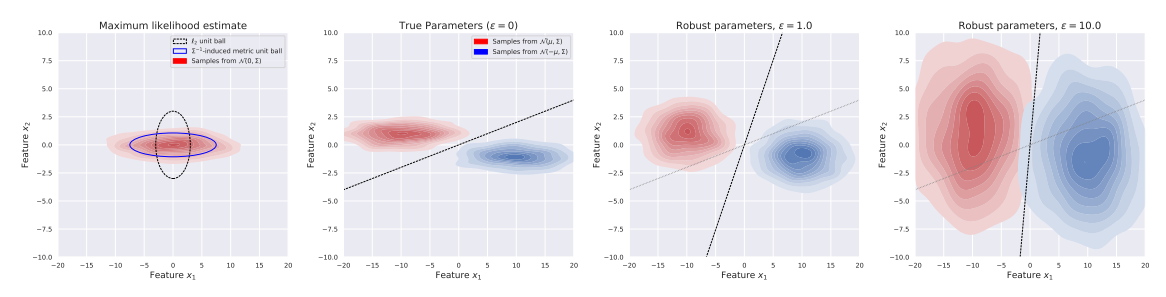
\includegraphics[width=13cm]{fig/figure4.png}
  \caption{定理2的效果的一个经验上的演示——当对抗扰动的幅度$\epsilon$增加时,学习到的$\mu$依然是常数,然是学习到的协方差与单位矩阵“融合”,有效地增加了非鲁棒特征上的不确定性。}
  \label{figure:4}
\end{figure}

\ \ \ \ 实际上,这样的一个不一致性恰好归咎于非鲁棒特征的存在,因为它在敌人的度量下沿着某个特定方向的“小”改变可以导致在由参数构建的数据依赖的距离上的一个大改变。如图\ref{figure:4}所示,特征诱导的度量中的偏差导致相应分类问题中存在非鲁棒特征。

\textbf{(2)鲁棒学习。}最优(非鲁棒)的最大似然估计是$\Theta=\Theta^{*}$,因此标准MLE估计的脆弱性完全由真实的数据分布控制。以下定理刻画了所学习到的参数在鲁棒问题中的行为。事实上,我们可以证明,在内部最大化上执行梯度下降(又名对抗训练)可以精确地得到 $\Theta_{r}$ 。我们发现,随着扰动幅度$\epsilon$的增加,学习到的特征诱导的度量混合了$\ell_{2}$度量和特征诱导的度量。

\textbf{定理2}(鲁棒地学习到的参数)。\textit{就像在非鲁棒的情形下一样,$\mu_{r}=\mu^{*}$,例如,真实的均值被学习到。对于鲁棒协方差$\Sigma_{r}$,存在一个$\varepsilon_{0}>0$,使得对任何一个$\varepsilon \in\left[0, \varepsilon_{0}\right)$,}
\begin{equation*}
  \Sigma_{r}=\frac{1}{2} \Sigma_{*}+\frac{1}{\lambda} \cdot I+\sqrt{\frac{1}{\lambda} \cdot \Sigma_{*}+\frac{1}{4} \Sigma_{*}^{2}}, \quad \text { where } \quad \Omega\left(\frac{1+\varepsilon^{1 / 2}}{\varepsilon^{1 / 2}+\varepsilon^{3 / 2}}\right) \leq \lambda \leq O\left(\frac{1+\varepsilon^{1 / 2}}{\varepsilon^{1 / 2}}\right)
\end{equation*}

\ \ \ \ 在$\ell_{2}$-限制的敌人下的鲁棒优化的效果可视化在图\ref{figure:4}中。当$\epsilon$增加,学习到的协方差变得与单位矩阵更一致。例如,我们可以看到,尽管分类对于自然分类很有用,但分类器在某些方向上的敏感度较低。

\textbf{(3)梯度de 可解释性。}Tsipras等人[tsi+19]观察到鲁棒模型的梯度在语义上更有意义。结果表明,在我们的模型下,这种行为是定理2的直接后果。特别地,我们表明,所得到的鲁棒学习得到的参数导致线性分类器的梯度和连接两个分布的平均值的向量在$\ell_2$内积下更好地对齐(在最坏的情况下)。

\textbf{定理3}(梯度对齐)。\textit{设$f(x)$和$f_r(x)$分别为基于标准和$\ell_2$鲁棒极大似然分类诱导的线性分类器。对于鲁棒模型,分类器(相对输入)的梯度与连接类的向量之间形成的最大角度可以更小:}
\begin{equation*}
  \min _{\mu} \frac{\left\langle\mu, \nabla_{x} f_{r}(x)\right\rangle}{\|\mu\| \cdot\left\|\nabla_{x} f_{r}(x)\right\|}>\min _{\mu} \frac{\left\langle\mu, \nabla_{x} f(x)\right\rangle}{\|\mu\| \cdot\left\|\nabla_{x} f(x)\right\|}
\end{equation*}

\ \ \ \ 图\ref{figure:4}在两维的情况下展示了这个现象。在对抗训练之后,梯度方向(垂直于决策边界)在$\ell_2$内积下与均值之间的向量逐渐对齐。

\textbf{讨论。}我们的理论分析表明,不提供任何定量的对分类的好处,一种自然的方式来看待鲁棒优化的作用是强加先验于分类器所学习的特征。尤其是,与一个$\ell_2$限制的敌人进行训练,可以防止分类器严重依赖于导致与$\ell_2$度量不同的度量的特征。

\textbf{鲁棒性和精度。}请注意,在目前描述的设置中,鲁棒性可能与准确性矛盾,因为鲁棒训练阻止我们学习最精确的分类器(在[TSI+19]中得出了类似的结论)。然而,我们注意到有非常相似的设置,其中非鲁棒特征以同样的方式表现出来,但是具有完好的鲁棒性和准确性的分类器仍然是可以实现的。很明显,虽然有许多非常精确的分类器,但是任何标准损失函数都将学习一个精确但不鲁棒的分类器。只有当采用鲁棒训练时,分类器才能学习一个完全准确和完全鲁棒的决策边界。

\section{相关工作}

在之前的工作中,许多解释对抗样本的模型被提出,这些模型利用了从有限样本的过度拟合到高维统计现象的各种思想[Gil+18;fff18;for+19;tg16;sha+19a;mdm18;sha+19b;gss15;bpr18]。我们模型的关键区别在于,对抗扰动是由泛化性好却脆弱的特征引起的,而不是统计异常或统计集中度差的影响。尤其是,由于第3.1节中关于“鲁棒化”数据分布的标准训练产生了鲁棒模型,因此对抗脆弱性并非源于使用特定的模型类或特定的训练方法。同时,如第3.2节所示,这些非鲁棒特征足以学习一个好的标准分类器。

\section{结论}

在这项工作中,我们将对抗样本的现象视为标准ML数据集中存在高度预测性但非鲁棒特征的自然结果。我们通过明确地分离标准数据集中的鲁棒和非鲁棒特征来支持这一假设,并表明仅非鲁棒特征就足以进行良好的泛化。最后,我们在一个理论环境中更详细地研究这些现象,在这个环境中我们可以严格地研究对抗脆弱性、鲁棒训练和梯度对齐。

\ \ \ \ 我们的发现促使我们把对抗样本根本上视为一种人类现象。特别是,我们不应该惊讶于分类器利用了高度预测的特征,这些特征恰好在人类选择的相似性概念下是非鲁棒的,而这些特征存在于现实数据集中。同样,从可解释性的角度来看,只要模型依赖于这些非鲁棒特征,我们就不能期望模型的解释既具有人类认为的意义又忠实于模型本身。总的来说,要获得鲁棒且可解释的模型,就需要在训练过程中明确地编码人类的先验知识。


\bibliographystyle{plain}
\bibliography{regularizations}

\end{document}
